Según se entra en la interfaz visual, el primer encuentro del usuario con la misma es la pantalla que se puede ver en la Figura \ref{fig:gui-completa}
\begin{figure}[H]
    \centering
    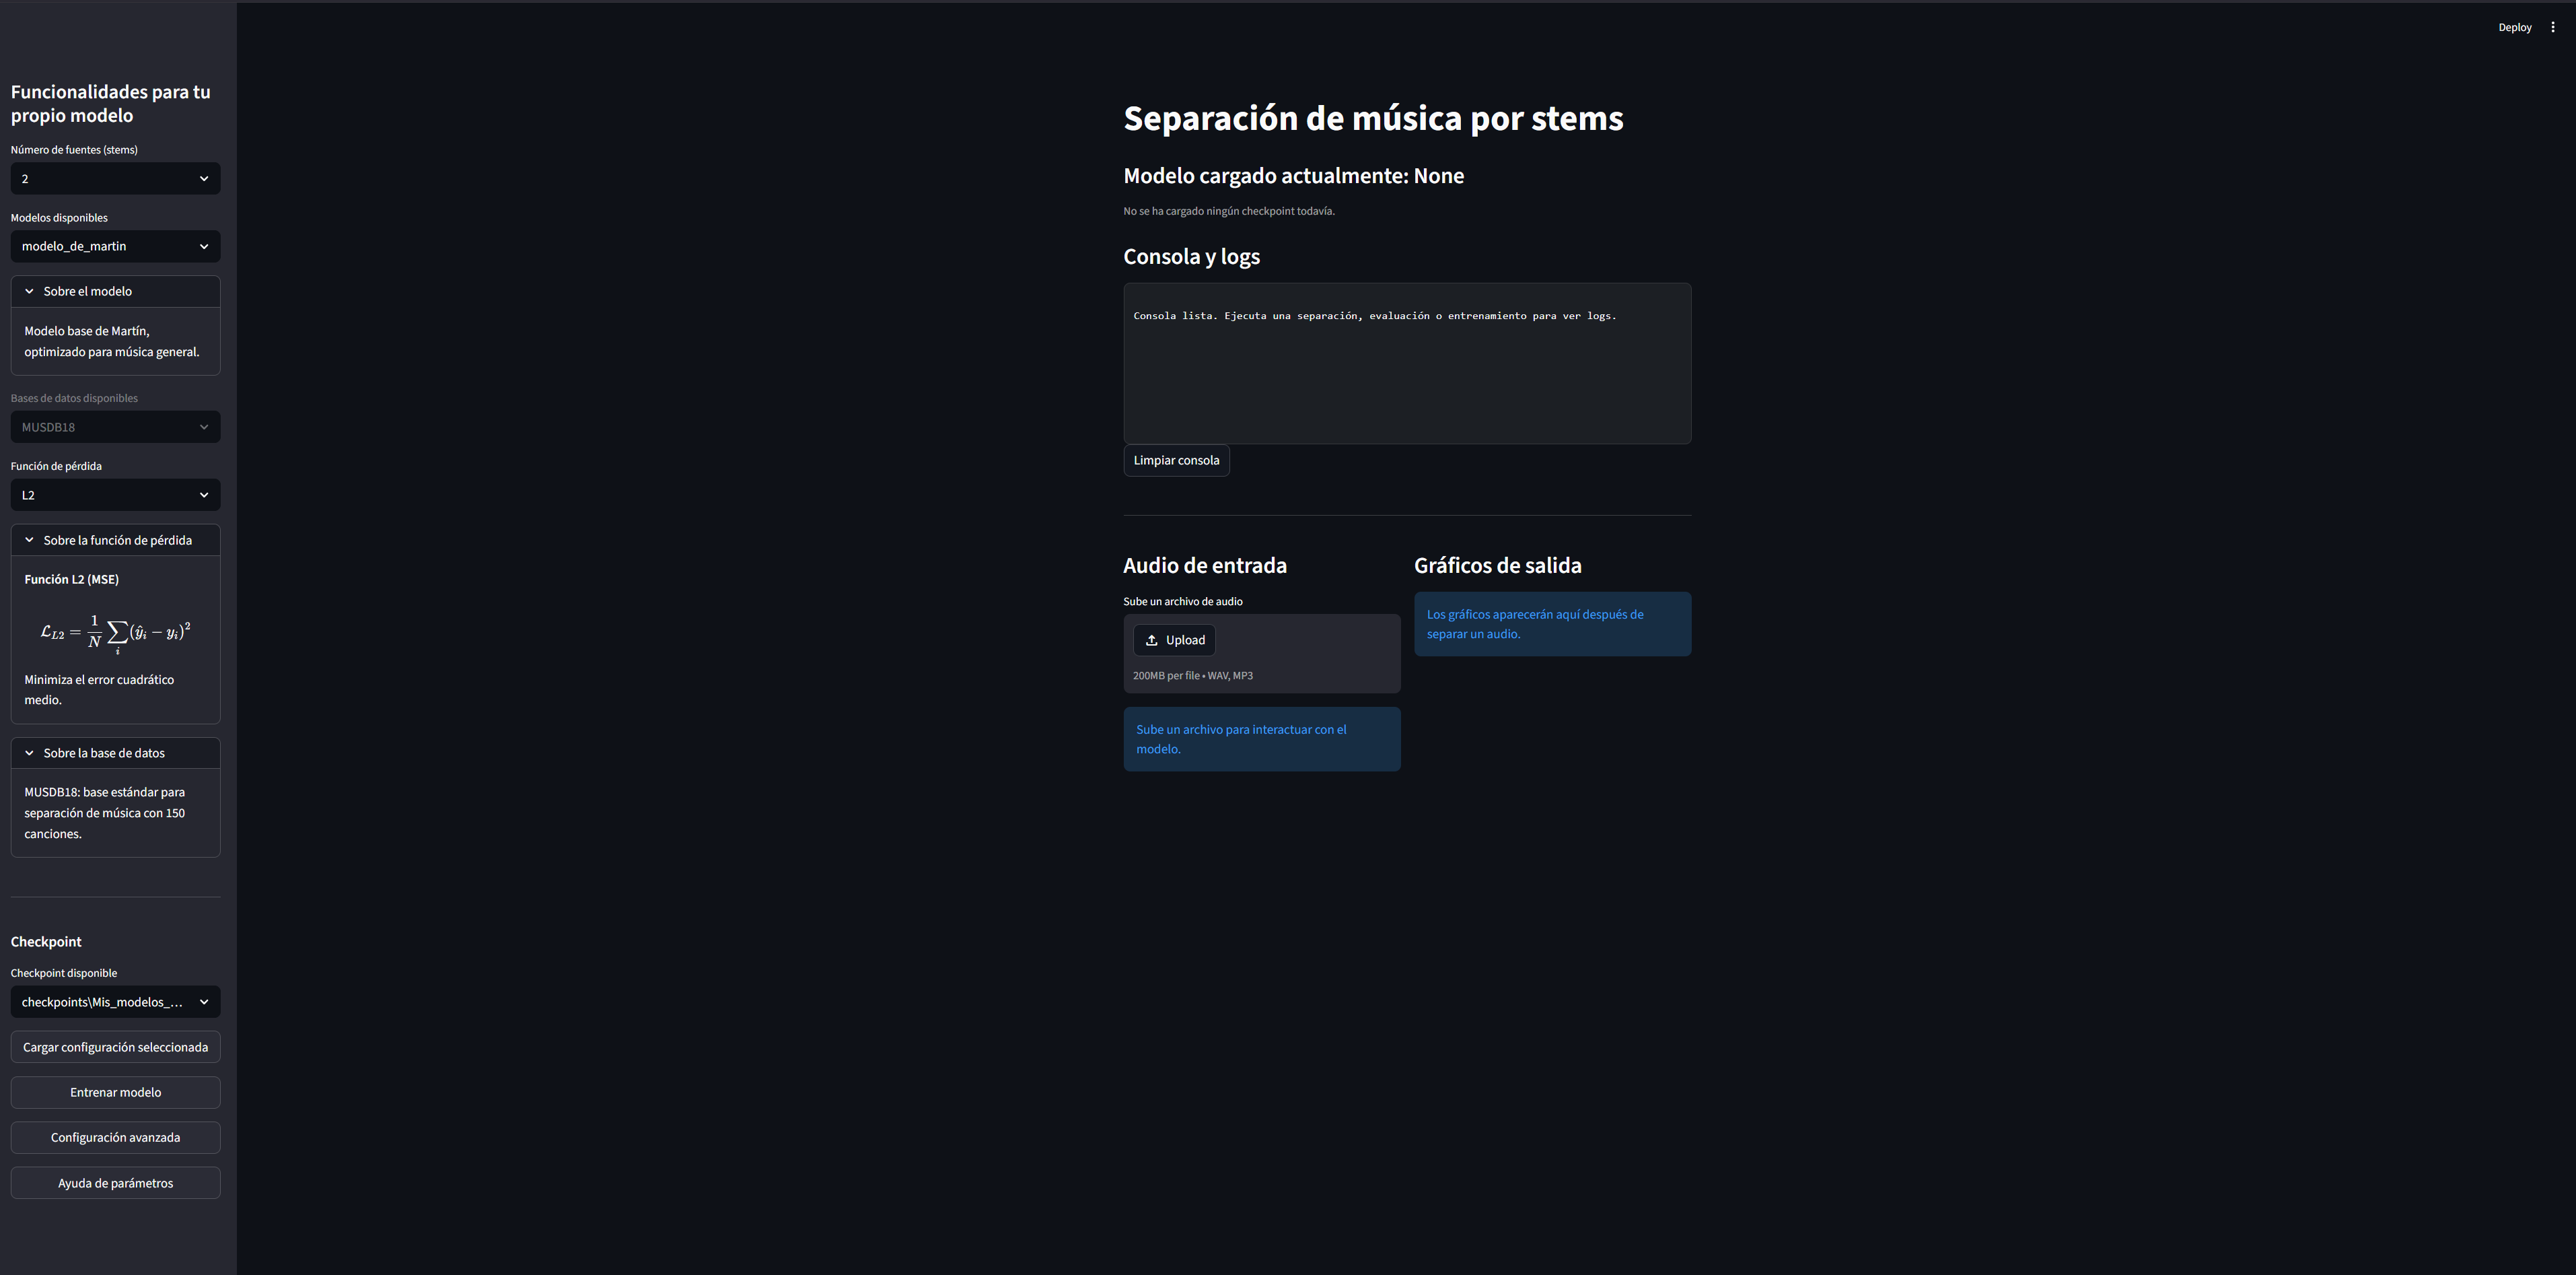
\includegraphics[width=0.75\textwidth,height=0.45\textheight,keepaspectratio]{commons/GUI_completa.png}
    \caption{Consola y logs de la GUI.}
    \label{fig:gui-completa}
\end{figure}

Posteriormente se diferencian los siguientes elementos:

\subsubsection{Barra lateral de configuración}
Se puede apreciar en la imagen de la Figura \ref{fig:gui-completa}.

La barra lateral permite seleccionar el número de fuentes, el modelo disponible, la base de datos, la función de pérdida y el checkpoint que se desea cargar.

\clearpage
\subsubsection{Zona principal de carga.}
Se permite subir un archivo de audio y lanzar el proceso de separación en la sección que se muestra en la Figura \ref{fig:zona-principal-gui}

\begin{figure}[H]
    \centering
    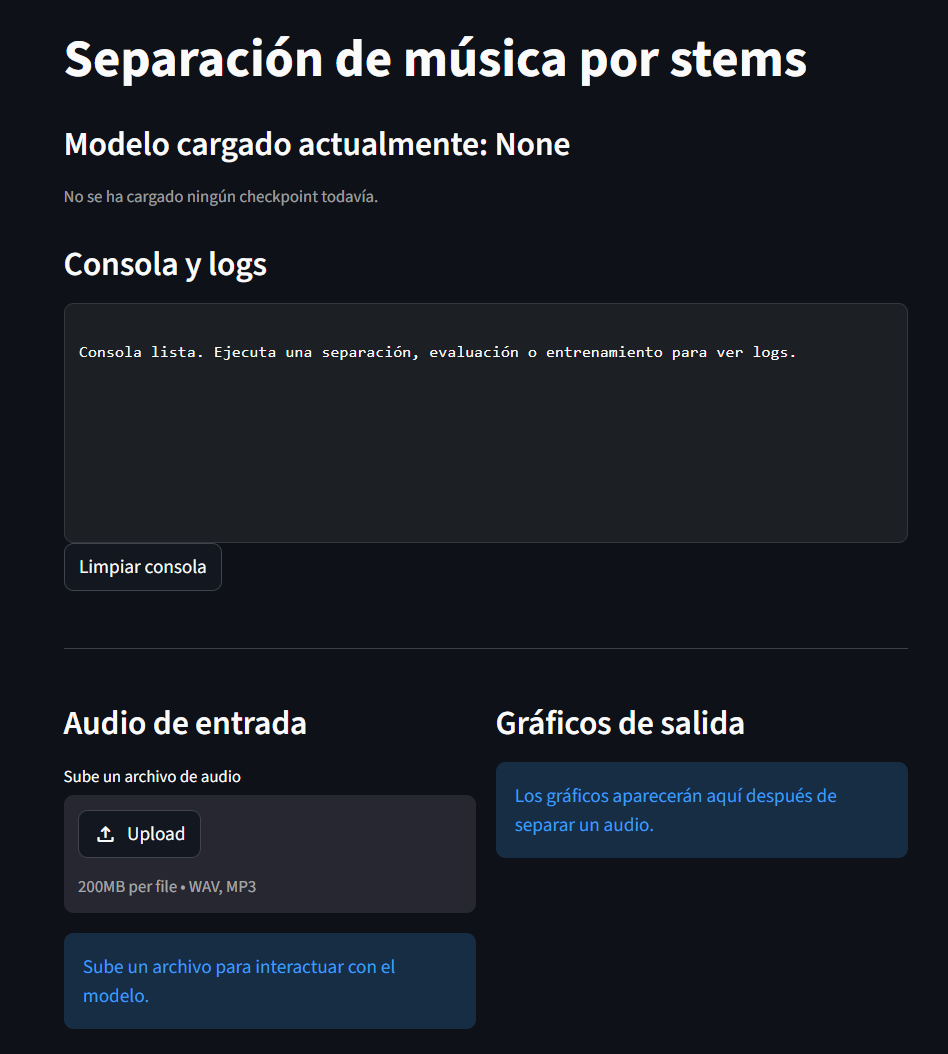
\includegraphics[width=0.75\textwidth,height=0.45\textheight,keepaspectratio]{commons/ZonaCarga_GUI.png}
    \caption{Zona principal de carga de la GUI.}
    \label{fig:zona-principal-gui}
\end{figure}

\subsubsection{Consola y logs.}
En la sección que se muestra en la Figura \ref{fig:consola-gui} se imprime en pantalla información sobre la ejecución del sistema, incluyendo mensajes de carga, separación, evaluación y posibles errores.

\begin{figure}[H]
    \centering
    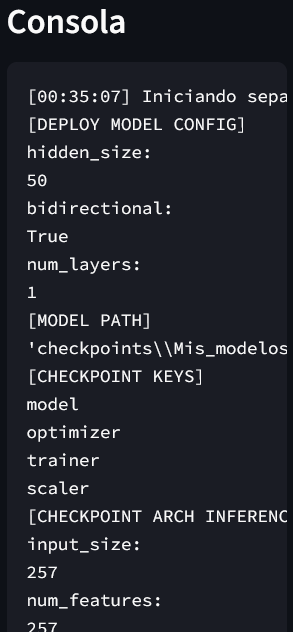
\includegraphics[width=0.75\textwidth,height=0.45\textheight,keepaspectratio]{commons/Consola_GUI_2.png}
    \caption{Consola y logs de la GUI.}
    \label{fig:consola-gui}
\end{figure}

\FloatBarrier

\subsubsection{Reproductores.}
Tras la separación, la interfaz muestra reproductores de audio para la mezcla original y para cada una de las fuentes separadas. 

Hay un reproductor para la mezcla original, ver Figura \ref{fig:reproductor-mezcla} y uno para cada fuente separada ya sea la separación de dos o de cuatro fuentes, ver Figuras \ref{fig:reproductor-vocales}, \ref{fig:reproductor-bajo}, \ref{fig:reproductor-bateria} y \ref{fig:reproductor-otros}.

\begin{figure}[H]
    \centering

    \begin{subfigure}{0.45\textwidth}
        \centering
        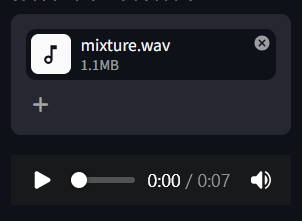
\includegraphics[width=\textwidth,height=0.16\textheight,keepaspectratio]{commons/Reproductor1_GUI.png}
        \caption{Mezcla original.}
        \label{fig:reproductor-mezcla}
    \end{subfigure}
    \hfill
    \begin{subfigure}{0.45\textwidth}
        \centering
        
\includegraphics[width=\textwidth,height=0.16\textheight,keepaspectratio]{commons/Reproductor2_GUI.png}
        \caption{Vocales.}
        \label{fig:reproductor-vocales}
    \end{subfigure}

    \vspace{0.3cm}

    \begin{subfigure}{0.45\textwidth}
        \centering
        
\includegraphics[width=\textwidth,height=0.16\textheight,keepaspectratio]{commons/Reproductor3_GUI.png}
        \caption{Bajo.}
        \label{fig:reproductor-bajo}
    \end{subfigure}
    \hfill
    \begin{subfigure}{0.45\textwidth}
        \centering
        
\includegraphics[width=\textwidth,height=0.16\textheight,keepaspectratio]{commons/Reproductor4_GUI.png}
        \caption{Batería.}
        \label{fig:reproductor-bateria}
    \end{subfigure}

    \vspace{0.3cm}

    \begin{subfigure}{0.45\textwidth}
        \centering
        
\includegraphics[width=\textwidth,height=0.16\textheight,keepaspectratio]{commons/Reproductor5_GUI.png}
        \caption{Otros.}
        \label{fig:reproductor-otros}
    \end{subfigure}

    \caption{Reproductores de audio de la interfaz.}
    \label{fig:reproductores-gui}
\end{figure}


\clearpage
\subsubsection{Gráficos.}
La interfaz también permite visualizar representaciones gráficas de las fuentes separadas, como la forma de onda y el espectrograma en las secciones que se muestran en la Figura \ref{fig:graficos-gui}.

\begin{figure}[H]
    \centering
    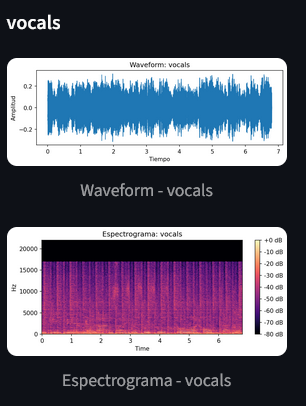
\includegraphics[width=0.85\textwidth,height=0.55\textheight,keepaspectratio]{commons/Graficos_GUI.png}
    \caption{Ejemplo de representación gráfica de la fuente vocal.}
    \label{fig:graficos-gui}
\end{figure}

\clearpage
\subsubsection{Botones.}
Se incluyen además botones para lanzar la separación, ver Figura \ref{fig:botones-gui}, evaluar el modelo, ver Figura \ref{fig:botones-gui-2}, y descargar los audios generados, ver Figura \ref{fig:botones-gui-3}.

\begin{figure}[H]
    \centering

    \begin{subfigure}{0.45\textwidth}
        \centering
        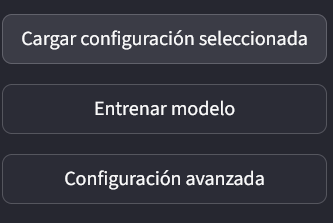
\includegraphics[width=\textwidth,height=0.16\textheight,keepaspectratio]{commons/Botones1_GUI.png}
        \caption{Botón de separación.}
        \label{fig:botones-gui-1}
    \end{subfigure}
    \hfill
    \begin{subfigure}{0.45\textwidth}
        \centering
        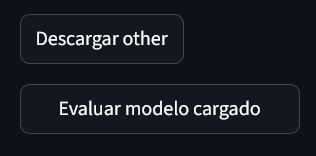
\includegraphics[width=\textwidth,height=0.16\textheight,keepaspectratio]{commons/Botones2_GUI.png}
        \caption{Botón de evaluación.}
        \label{fig:botones-gui-2}
    \end{subfigure}

    \vspace{0.3cm}

    \begin{subfigure}{0.45\textwidth}
        \centering
        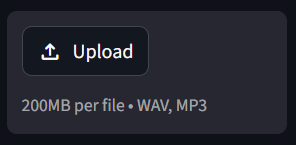
\includegraphics[width=\textwidth,height=0.16\textheight,keepaspectratio]{commons/Botones3_GUI.png}
        \caption{Botón de descarga.}
        \label{fig:botones-gui-3}
    \end{subfigure}
    \hfill
    \begin{subfigure}{0.45\textwidth}
        \centering
        
\includegraphics[width=\textwidth,height=0.16\textheight,keepaspectratio]{commons/Botones4_GUI.png}
        \caption{Botón auxiliar.}
        \label{fig:botones-gui-4}
    \end{subfigure}

    \caption{Botones principales de la interfaz.}
    \label{fig:botones-gui}
\end{figure}

